\begin{tcolorbox}[posterbox]
\SectionTitle{Theoretical Overview}

Dual-systems theories propose a \textbf{Parallel Individuation (PI)} system for small sets (1-3) and an \textbf{Approximate Number System (ANS)} for larger sets (4+).
\begin{itemize}
  \item Passive EEG work showed N1 scaling for small numerosity (Hyde \& Spelke, 2012).
  \item Active change detection effects for direction and distance are less understood.
  \item We test frontal MMN-like and posterior N1 signatures in one active paradigm.
\end{itemize}
\end{tcolorbox}

\vspace{0.14in}

\begin{tcolorbox}[posterbox]
\SectionTitle{Study Design and Procedure}

\SmallText
\begin{itemize}
  \item \textbf{Participants:} N=24 right-handed adults.
  \item \textbf{Stimuli:} non-symbolic arrays 1-6 (area/luminance controlled).
  \item \textbf{Timing:} 250 ms stimulus duration, 750-1250 ms jittered ISI.
  \item \textbf{Prime/target:} 3-5 prime repeats, then no-change, within-range, or crossover target.
  \item \textbf{Task:} participants actively detected changes and responded by key press.
\end{itemize}

\begin{center}
  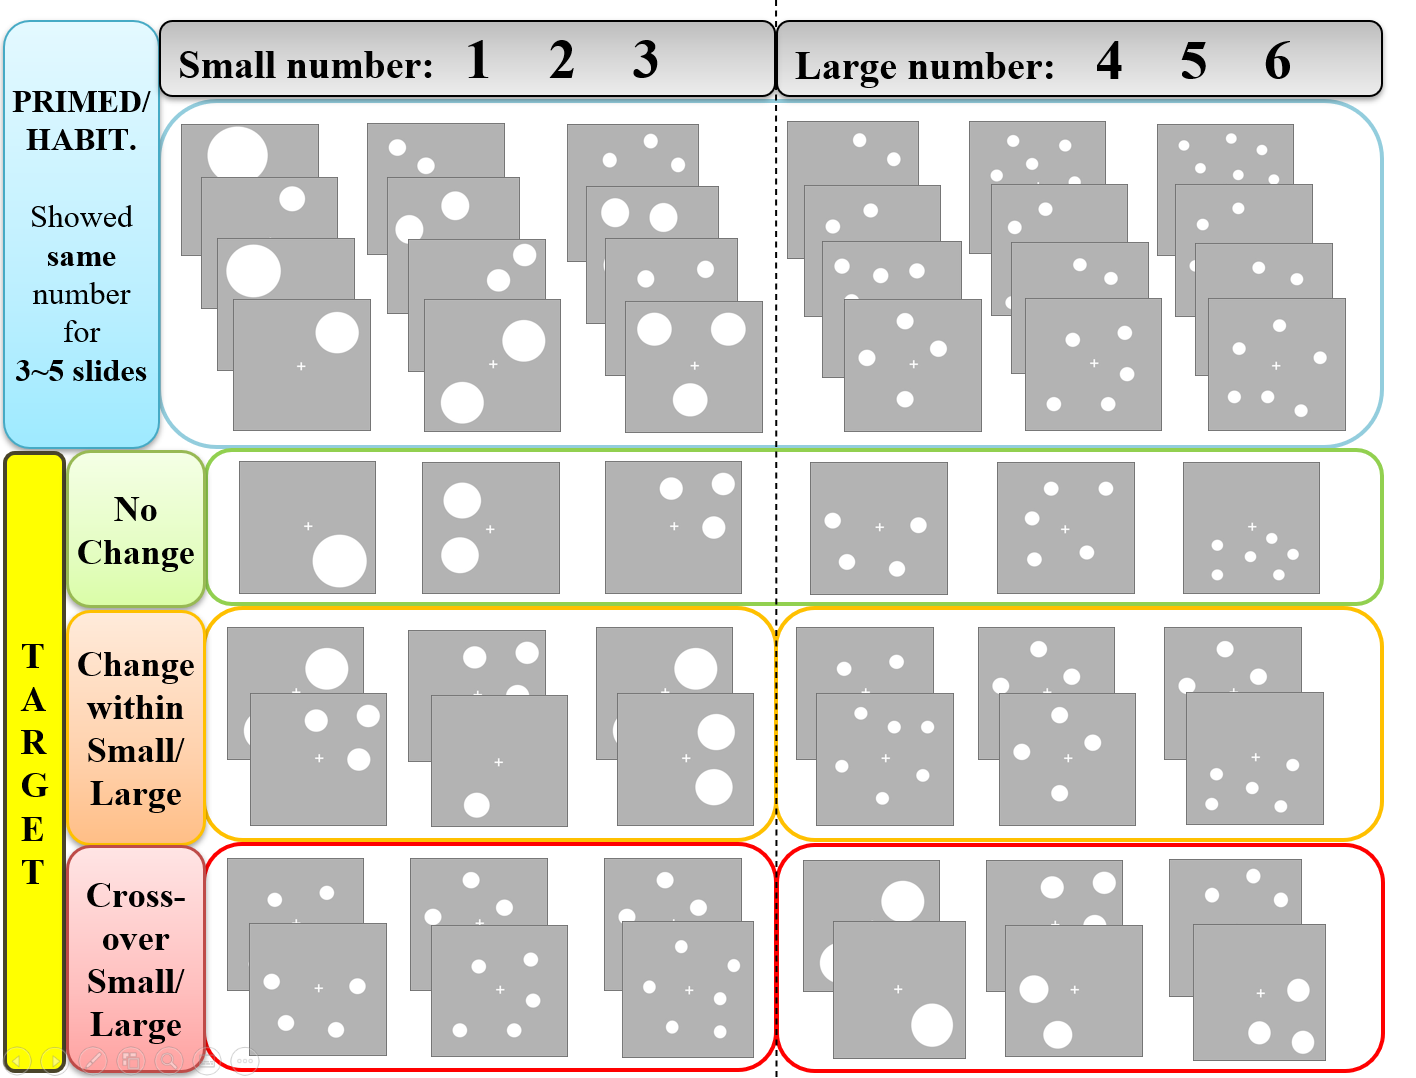
\includegraphics[width=0.82\linewidth]{media/stimuli_presentation.png}
\end{center}
\SmallText
\textbf{Fig. 1.} Active change-detection paradigm and example numerosity transitions.
\end{tcolorbox}
